\newlength{\bibsep}
\documentclass[nonatbib,5p,a4paper]{elsarticle}  % 5p for two columns, 1p for 1 column (this is specific for the elsearticle)
\usepackage[english,norsk,nynorsk]{babel}        % Language
\usepackage[DatePublished]{Code/NTNU-lab}        % remove [DatePublished] to remove dates
\usepackage{csquotes}                            % Must be loaded when babel is loaded to avoid error.
% Use this file to write code that you do not want in the .sty file, but has to be in the preamble (before \begin{document}).
% Writing in this file in stead of in the preamble will keep the main file more organised and tidy.


%                       Nomenclatures
%_______________________________________________________________
\usepackage[intoc]{nomencl}
\makenomenclature
\usepackage{listings}
\renewcommand{\nomname}{%
% Title
%----------------
List of Symbols
%----------------
}
\renewcommand{\nompreamble}{%
% Description
%----------------
The next list describes several symbols that will be later used within the body of the document
%----------------
}
% This code creates the groups
\renewcommand\nomgroup[1]{%
  \item[\bfseries
  \ifstrequal{#1}{A}{Physics constants}{%
  \ifstrequal{#1}{B}{Mathematical constants}{%
  \ifstrequal{#1}{C}{Other symbols}{}}}%
]}
% This will add the units
\newcommand{\nomunit}[1]{%
\renewcommand{\nomentryend}{\\#1}}
%................................................................

                            % Write all preamble code in this file to keep it organised and tidy.

\addbibresource{Bibliography/Sources.bib}        % Selects the Bibliography file.


\begin{document}
\selectlanguage{english}                         % Sets the language of the document.

%%%%%%%%%%%%%%%%%%%%%%%%%%%%%%%%%%%%%%%%

\begin{frontmatter}
%
% Title:
%------------------------------------
\title{%
Final Report\\
\small For individual project  % A good idea is to have the subject code and name as subtitle
}
%
% Authors:
%------------------------------------
% List an author with name ' Firstname Middlename Lastname ' like this:
% F. M. Lastname
\author{Jonas Brami} 
\author{Brett Stevens}

%
% Date:
%------------------------------------
%
\newdate{dateName}{31}{08}{2022} % edit the date here, ' dateName ' has to match on these two lines.
\renewcommand*{\today}{\DayMonthYearDateFormat\displaydate{dateName}} 
% Options for displaying date: \MonthYearDateFormat,  \DayMonthYearDateFormat or \YearDateFormat
%
% Abstract:
%------------------------------------
%
\end{frontmatter}
%
%
% Table of contents:
%------------------------------------
% If the report is very long for some reason (over 4 or 5 pages), use a table of contents.
% Uncomment everything below the line ---- to get table of contents (ctrl + /) (the / on numberpad):
%-------------

\ 
\vspace{1cm}

\begin{minipage}{\textwidth}
    \tableofcontents
\end{minipage}
\clearpage
\section{Introduction}
% Delete the text and write your Introduction here:
%------------------------------------




The problem we aim to solve during this project is the placement of a sensor on a specific target point on a surface using a fixed manipulator arm mounted on the top of an unmanned quadcopter.
A quacopter is an underactuacted helicopter with four rotors. This UAV (Unmanned Aerial Vehicles) is underactuated because arbitrary configurations and trajectory cannot be realized.\\
In the last ten years, research about UAV controls accelerated drastically with many applications in the civilian industry in a variety of areas.\\
Monitoring and sensing tasks are traditionally operated by human but they be complicated, expensive and dangerous for the human operator when the point of interest is hard to reach. For example, big structures like bridges need to undergo regular inspections to ensure there are no cracks or other signs of structural fatigue.\\
Using UAVs for such tasks would not only reduce cost of maintance of those structures, but also increase the security of both the human manipulator and the civilians using it. \\
Sensor placement on surfaces using UAVs  is an active field of research and we will propose a solution based on velocity fields.\\

A velocity field is a function taking as input  a four dimensional vector $(x,y,z,t)$ and returning a 3 dimensional velocity vector $(u,v,w)$.\\
Since our environment is static, meaning that the obstacles and goal are not moving, we will always use a time invariant velocity field.
Diverse ways of placing sensors using UAVs have been explored in the past, including but not limited to: 
\begin{itemize}
    \item Direct Placement: Using a fixed arm manipulator on an UAV, we use the force exerted by the thrust of the UAV to provide enough pressure on the tip of the arm to place the sensor on the target point.
    \item Sensor Launching \cite{farinha2020unmanned}: Using the energy stored in a spring, the UAV ejects the sensor at the desired velocity to reach and attach to the target (Unmanned Aerial Sensor Placement for Cluttered Environments). This strategy is very useful when it is not physically possible for a mounted arm to reach the target however it suffers from small payload capacity.
    \item Drop from flight: We simply drop the sensor above the target point. When target accuracy is not a priority and we are aiming at a non-vertical surface and there is no occlusion above the target,  this sensor placement strategy is the most effective. 
\end{itemize}
\begin{figure}[h!]
    \centering
    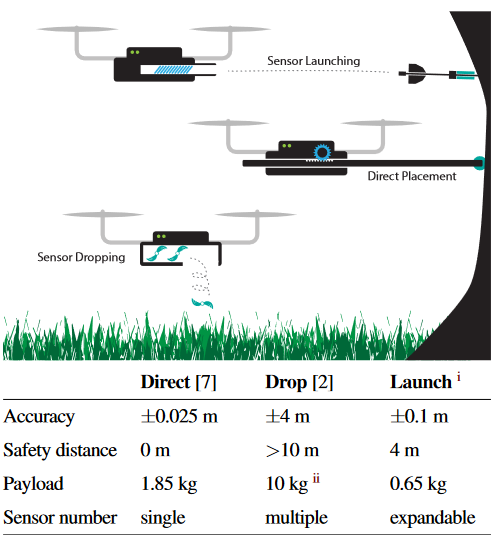
\includegraphics[width=0.48\textwidth]{Images/threeway.png}
    \caption{Different types of sensor placement from \cite{farinha2020unmanned}}
    \label{fig:threeway}
\end{figure}
The characteristics of each one of mentioned methods are shown in \ref{fig:threeway}.
We decided to go through with the Direct Placement strategy because despite its simplicity, it provides good accuracy and is able to place a large variety of payloads. 
The solution we will propose can be divided in 3 parts: The first is environment mapping where we perform surface and obstacle recognition using live depth sensor feed. The second part is designing a potential based velocity field to perform path-planning by guiding the UAV from the start point to the target point. The third and last part is designing a velocity field around the target point to apply the desired force amplitude. In this part, we will use the passive velocity field controller (PVFC) to optimize our energy consumption.

\section{Literature Review and Theory}
% Delete the text and write your Theory/ Background Information here:
%------------------------------------
1- PVFC
2- Potential field
3- Asl Narikiyo ? no countour so no need?
\subsection{Velocity field path-planning for single and multiple unmanned aerial vehicles}
In the paper "Velocity field path-planning for single and multiple unmanned aerial vehicles", the author presents a path-planning technique based on Velocity Fields generated from potentials solution of Laplace's equation.
Two different type of solution to the Laplace 
\begin{align} % Use & sign to align, use \nonumber to write a line without number.
    \laplacian{V} &=0 \nonumber \\
    \frac{\partial^2 V}{\partial x^2}+\dpd[2]{V}{y} &=0 \label{eq:Laplace} % dpd = display mode partial derivative
\end{align}
equation are presented in this paper: Type 1 are irrotational solutions to generate sink and source fields and Type 2 solution are used to build solenoidal fields.
\begin{align} % Use & sign to align, use \nonumber to write a line without number.
    {V}_{1} = {Q}_{1} \ln(({x}_{1}-\tilde{{x}_{1}})^2+({x}_{2}-\tilde{{x}_{2}})^2) \\
    {V}_{2} = {Q}_{2} \arctan(\frac{({x}_{2}-\tilde{{x}_{2}})}{({x}_{1}-\tilde{{x}_{1}})})
\end{align}
$({x}_{1},{x}_{2})$ is the position of the UAV\\
$(\tilde{{x}_{1}}, \tilde{{x}_{2}})$ is the position of the obstacle\\
${V}_{1}$ and ${V}_{2}$ are respectively type 1 solution (source field) and type 2 solution (vortex field). \\
The author justifies the use of Laplace solution for building the velocity field for multiple reasons:
\begin{itemize}
    \item The use of Laplace solution for potential guaranties the uniqueness of minimum in the field. 
    Specifically, the use of vortex function built from shaping function to circle around obstacle will.
    This ensures that only the goal point will be a minimum and that the UAV will not get stuck at some local minimum. 
    As the author states, we can do an analogy with a famous strategy to find the exit of a maze: 
    By keeping a hand on a wall of the maze and walking while always touching the wall, we are ensured to find the end of the maze. 
    This is far from being an optimal solution, however, by using vortex function to circle around obstacle, we can provide the guaranty that the goal will be reached. 
    As a result, those solenoidal fields based on vortex function also provides active collision avoidance. 
    \item Scalar shaping functions are at the base of these methodology because by crafting them to match the shape of the obstacles, 
    we are able to generate corresponding vortex functions for obstacles of any shape. 
    Since the vortex field is defined for each obstacle, it would be easy to reevaluate the field add/removal of an obstacle.
    \item Finally, irrotational solutions of the Laplace equation allows us the define an exclusion radius around obstacles (source field) and to direct ourself in direction of the target point (sink field).
    The exclusion radius is encoded using the amplitude ${Q}_{1}$ of the irrotational field.
\end{itemize}

We can leverage these both types of potentials to derive a velocity field that will guide the UAV to the contact point without colliding with the surface.
For example we could define the exclusion radius to be the distance between the centre of mass (CoM) of the quadcopter and its most distant part on the quadcopter. 
We will still be able to make contact because the distance between the tip of the arm and the CoM will be longer than this exclusion radius. 


\subsection{Spherical field to maintain desired force }
When contact has been made, we suppose that the surface static friction coefficient is high enough to maintain the contact.
Since the arm has a fixed size and does not move, this part will describe a partial sphere around the target point with a radius defined by the distance between the CoM of the quadcopter and the tip of the arm.
First we need to compute the feasible position of the CoM to apply the desired force. 
We know that this position is unique because there is only one vertically stable pitch for a given desired force amplitude. We can either compute this position analytically or we can use machine learning techniques such as regression to compute the feasible pitch in function of the desired force. The latter option would require collecting training data from simulations on gazebo. 
Now we can generate the velocity field on the surface of the sphere to point on the tangent direction of the sphere in the direction of the stable pitch position with an amplitude proportional to the distance from this point. Finally, we use the Passive Velocity Field Control to follow this field


\subsection{PVFC}

\subsection{Asl Narikiyo coutour}
normal + tangeant ? talk about it despite not doing countour

\section{Technical Experimentation}
In this section, we will present the field we previously described with illustrations. 
\begin{figure}[h!]
    \centering
    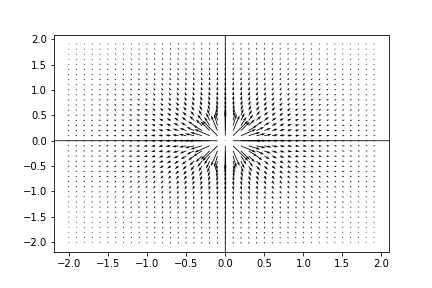
\includegraphics[width=0.48\textwidth]{Images/simplesource.png}
    \caption{Simple Type 1 irrotational source}
    \label{fig:simplesource}
\end{figure}
The field in figure \ref{fig:simplesource} was drawn by computing the gradient of $V_1$ with $(\tilde{{x}_{1}}, \tilde{{x}_{2}}) = (0,0)$.

\begin{figure}[h!]
    \centering
    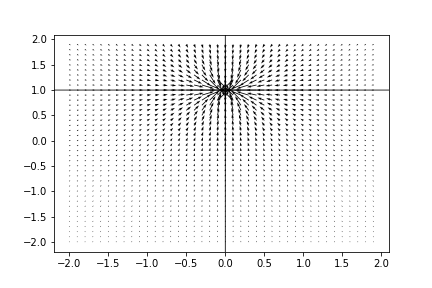
\includegraphics[width=0.48\textwidth]{Images/simplesink01.png}
    \caption{Simple Type 1 irrotational sink}
    \label{fig:simplesink}
\end{figure}
The field in figure \ref{fig:simplesink} is a sink field at $(0,1)$, it is similar to the source field in figure \ref{fig:simplesource} but with opposite sign.

\begin{figure}[h!]
    \centering
    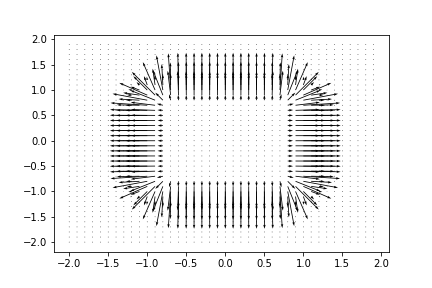
\includegraphics[width=0.48\textwidth]{Images/irrotafromshaping.png}
    \caption{irrotational field from shaping}
    \label{fig:irrotafromshaping}
\end{figure}
The field in figure \ref{fig:irrotafromshaping} has been generated by computing the gradient of the shaping function of a superquadratic: 
$F=\frac{1}{1+(\frac{1}{L}H^{\frac{1}{n}})^m}$ with $H=(x_1-\tilde{{x}_{1}})^n+(x_2-\tilde{{x}_{2}})^n$.
As stated in \cite{mcinnes2003velocity}, when $m\gg1$, the edge of the shaping function gets thinner. Higher values of $n$ result in more rectangular shapes whereas $n=2$ describes the shaping function of a sphere.

Both these fields are type 1 irrotational solutions of the Laplace equation.

By adding the irrotational sink from figure \ref{fig:simplesink} and the irrotational field from shaping function in figure \ref{fig:irrotafromshaping} we obtain a good representation in figure \ref{fig:irrotafromshapingwithsink} of what the velocity field will look like when close to the target point. 
\begin{figure}[h!]
    \centering
    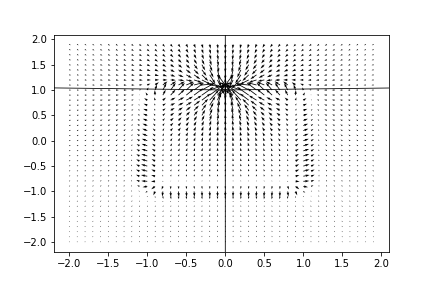
\includegraphics[width=0.48\textwidth]{Images/irrotashapingwithsink.png}
    \caption{irrotational field from shaping with sink}
    \label{fig:irrotafromshapingwithsink}
\end{figure}

The shaping function is mainly used to generate a vortex field around an obstacle, as explained in the paper. It is given by: 
$v_2=-\frac{\partial{F}}{\partial{x_2}}e_1 + \frac{\partial{F}}{\partial{x_1}}e_2 $.
We can see in figure \ref{fig:rotafromshaping} an example of vortex field around a super quadriatic.
\begin{figure}[h!]
    \centering
    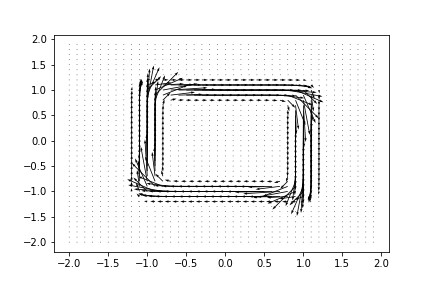
\includegraphics[width=0.48\textwidth]{Images/rotafromshaping.png}
    \caption{Solenoidale field from shaping function}
    \label{fig:rotafromshaping}
\end{figure}

As explained in section 2, after we made contact, we stop using the potential based field and we use the spherical field to maintain 
contact with the desired force. 
Figure \ref{fig:spherical} represents an example of such a field.
\begin{figure}[h!]
    \centering
    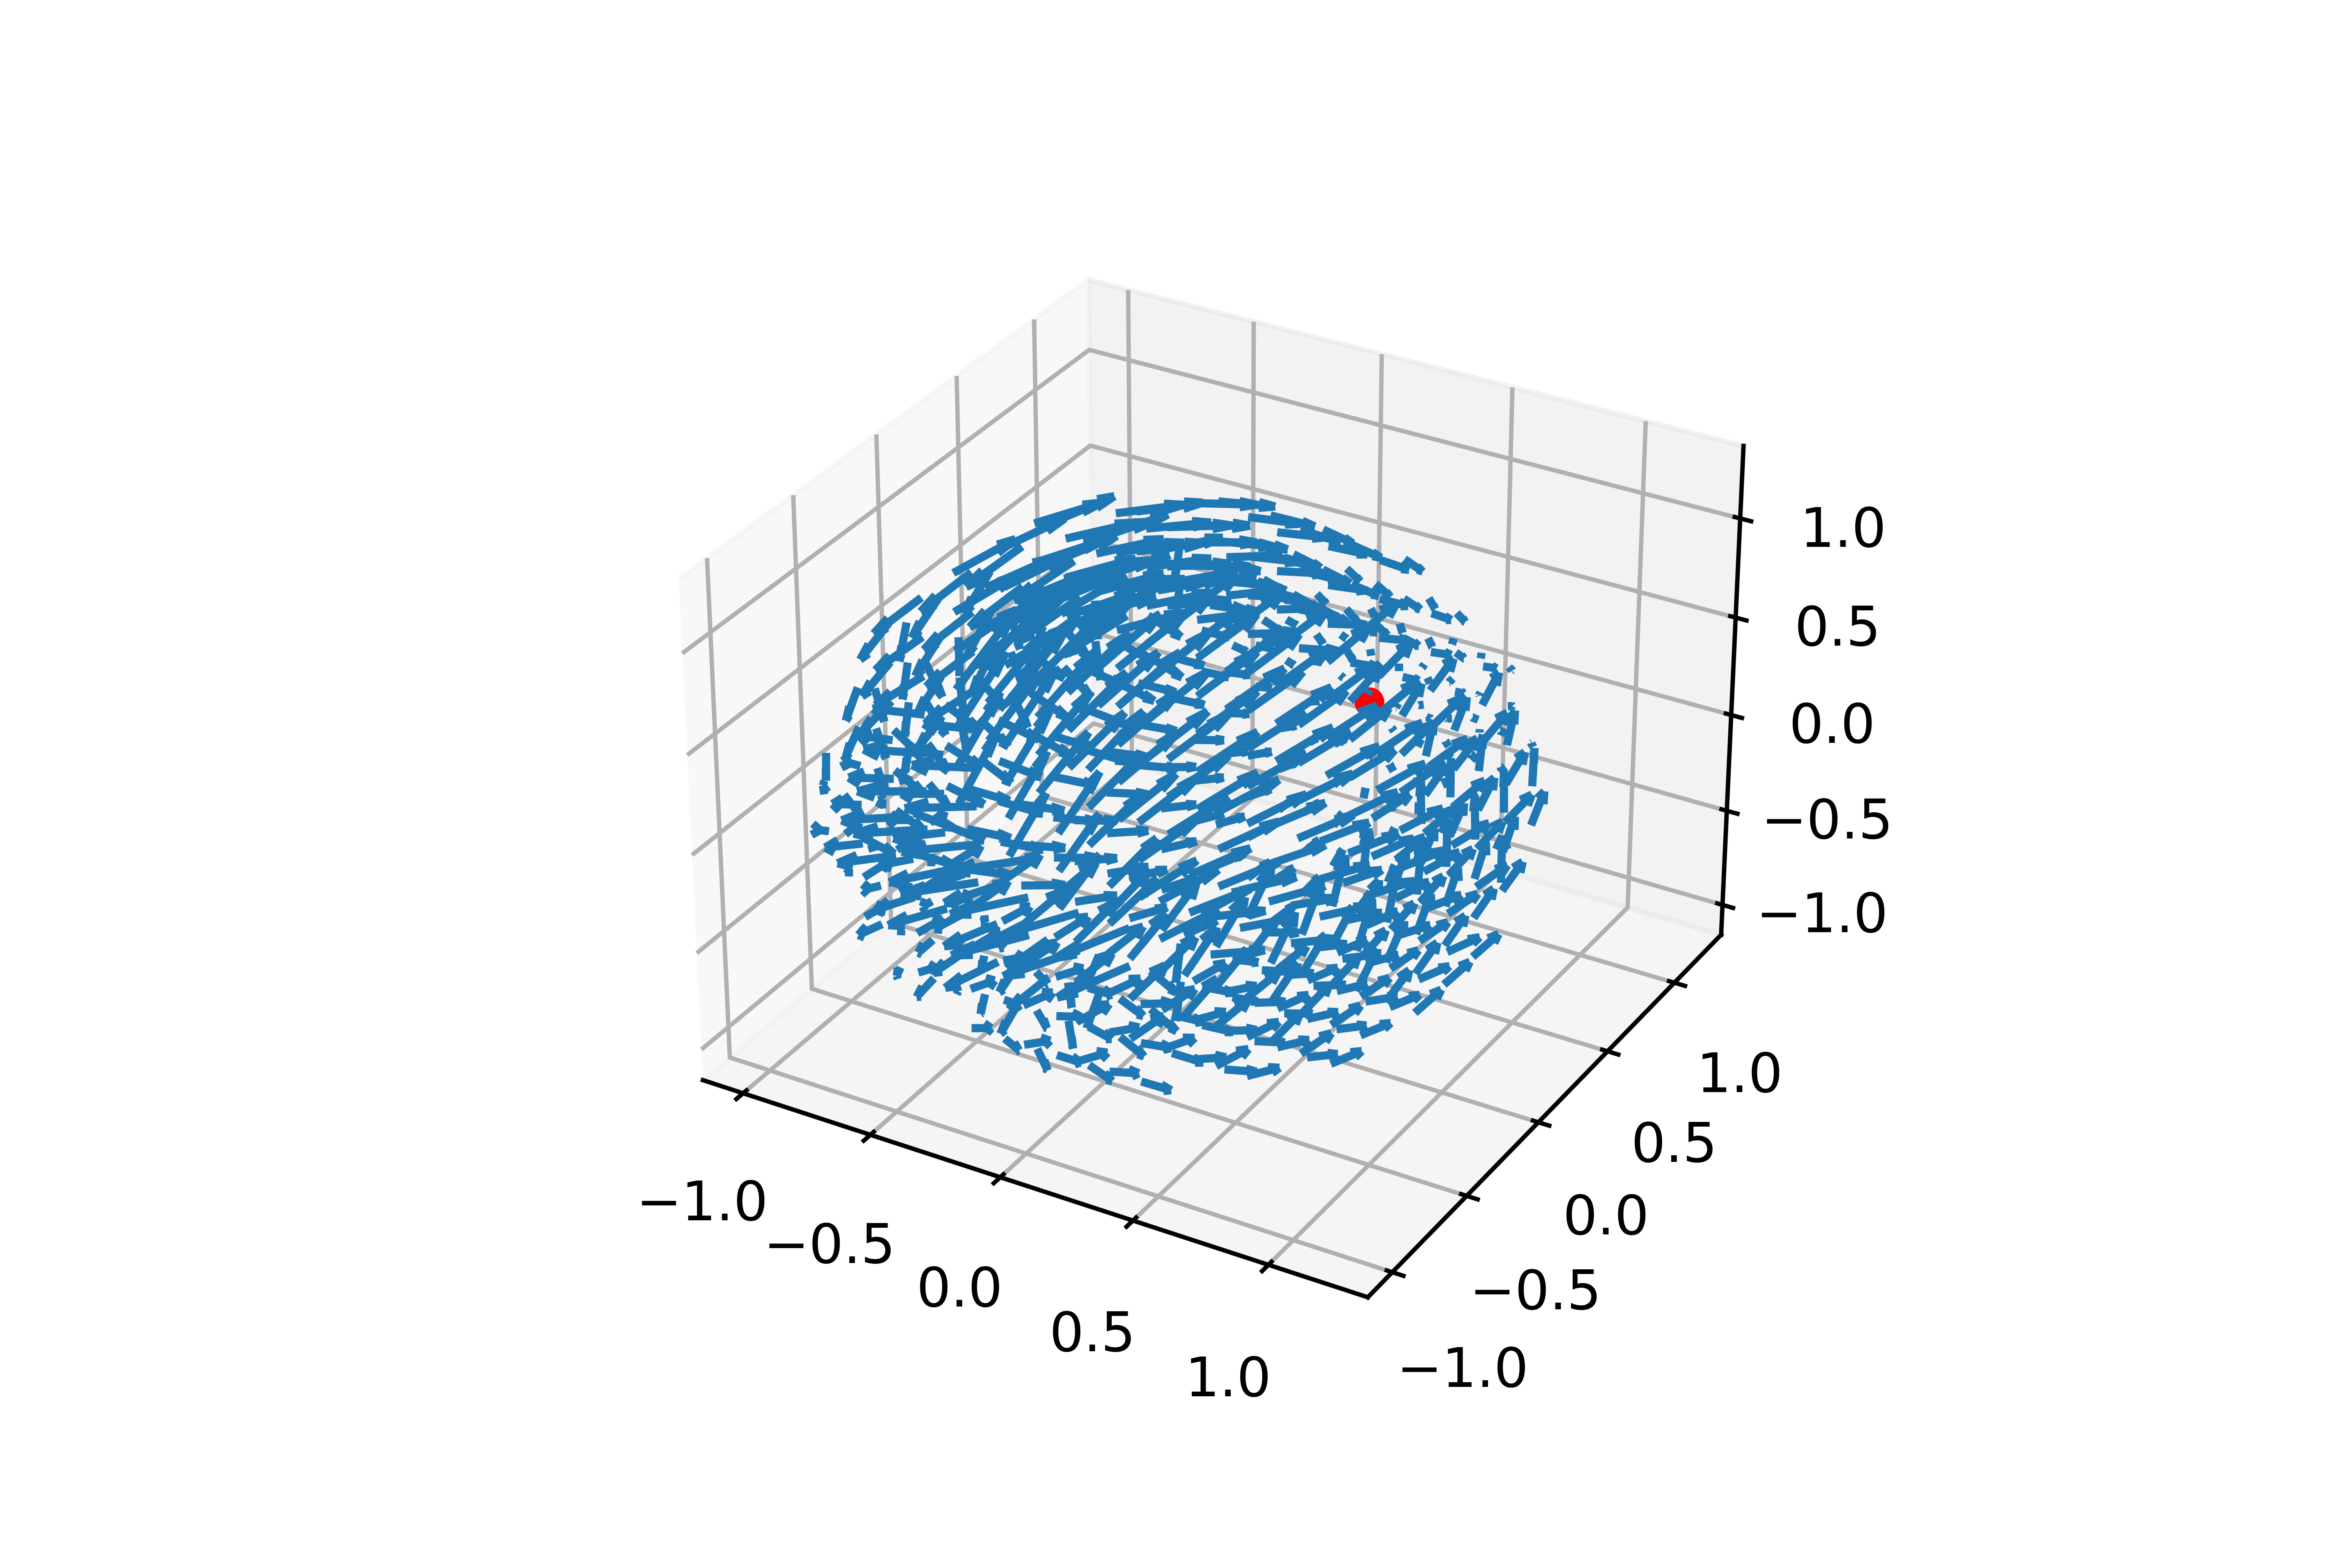
\includegraphics[width=0.48\textwidth]{Images/sphericalfield.png}
    \caption{Spherical contact field}
    \label{fig:spherical}
\end{figure}

\section{Project Plan}

\newpage
%\clearpage                                     % Sometimes you want the rest on separate pages.

%%%%%%%%%%%%%%%%%%%%%%%%%%%%%%%%%%%%%%%%

% Bibliography
%--------------------
\printbibliography

\end{document}

% Copyright Remarks:
%--------------------

% Copyright holder: Vebjørn S. Førde, copyright: CC BY 4.0
% Note: The author of this template is also the copyright holder.

% Below is an explanation of the CC BY 4.0. Additional statements/ 
% clarifications made by the author/copyright holder are marked with *.

% YOU ARE FREE TO:
% Share — copy and redistribute the material in any medium or format
% Adapt — remix, transform, and build upon the material
% for any purpose, even commercially.

% UNDER THE FOLLOWING TERMS:
% Attribution* — You must give appropriate credit, provide a link to the license,
% and indicate if changes were made. You may do so in any reasonable manner, but 
% not in any way that suggests the licensor endorses you or your use.

% *Note: I do not need credit when the template is used to make a PDF document
% that is then distributed (like handing in a lab report). However, I would
% like for you to give credit if you choose to distribute the "software" 
% (the associated documentation files, .tex files and such). If you distribute
% both the PDF and the software, then you only need to give credit in the software
% distribution.
% I do not need credit for the plain text (text in output PDF). However, you should
% give me credit if you chose to use/ distribute any of the images in this document.

% No additional restrictions — You may not apply legal terms or technological 
% measures that legally restrict others from doing anything the license permits.

% NOTICES:
% No warranties are given.

% Disclaimer* (added by copyright holder):
% THE SOFTWARE IS PROVIDED "AS IS", WITHOUT WARRANTY OF ANY KIND, EXPRESS OR
% IMPLIED, INCLUDING BUT NOT LIMITED TO THE WARRANTIES OF MERCHANTABILITY,
% FITNESS FOR A PARTICULAR PURPOSE AND NONINFRINGEMENT. IN NO EVENT SHALL THE
% AUTHORS OR COPYRIGHT HOLDERS BE LIABLE FOR ANY CLAIM, DAMAGES OR OTHER
% LIABILITY, WHETHER IN AN ACTION OF CONTRACT, TORT OR OTHERWISE, ARISING FROM,
% OUT OF OR IN CONNECTION WITH THE SOFTWARE OR THE USE OR OTHER DEALINGS IN THE
% SOFTWARE.

% Read more about CC BY 4.0:
% https://creativecommons.org/licenses/by/4.0/